\begin{figure}
\centering
    
% Define the legend

\begin{tikzpicture}
\centering
\begin{axis}[
    hide axis,
    xmin=0, xmax=10, ymin=0, ymax=0.4,
    legend style={
        draw=none,
        fill=none,
        legend columns=-1,
        /tikz/every even column/.append style={column sep=0.2cm},
        font=\tiny,
        at={(0.5,1.02)},
    },
    legend cell align={left},
]
\addlegendimage{red, const plot, thick, solid, mark=*}
\addlegendimage{blue, const plot, thick, dashed, mark=square*}
\addlegendimage{green, const plot, thick, dotted, mark=triangle*}
\addlegendimage{orange, const plot, thick, dashdotted, mark=diamond*}
\addlegendimage{purple, const plot, thick, loosely dashed, mark=pentagon*}
\addlegendentry{CASCADE}
\addlegendentry{FAST\_JITTERS}
\addlegendentry{INTRA\_CASCADE}
\addlegendentry{SLOW\_JITTERS}
\addlegendentry{SPIKE}
\end{axis}
\end{tikzpicture}

\bigskip

\begin{subfigure}{0.45\textwidth}
\centering
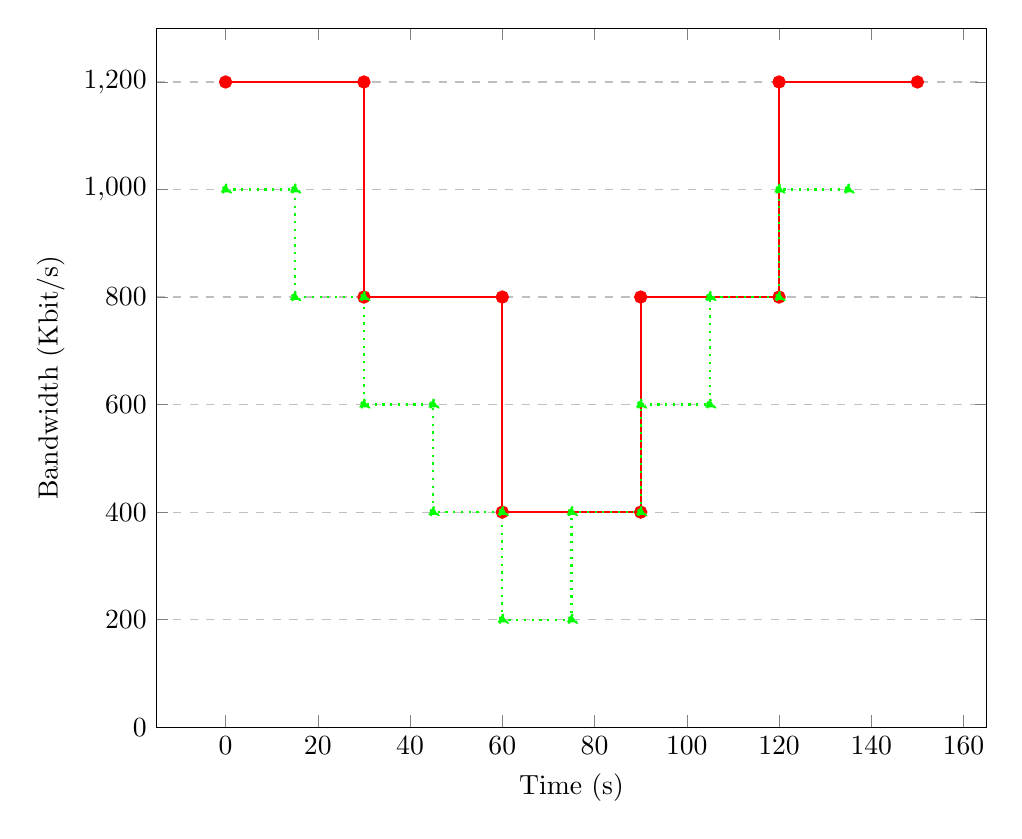
\begin{tikzpicture}
    \begin{axis}[
        width=\textwidth,
        xlabel={Time (s)},
        ylabel={Bandwidth (Kbit/s)},
        ymin=0, ymax=1300, ytick distance=200,
        ymajorgrids=true,
        grid style=dashed,
    ]
    
% CASCADE
\addplot[red, const plot, thick, solid, mark=*] coordinates {
    (0,1200) (30,1200) (30,800) (60,800) (60,400) (90,400)
    (90,800) (120,800) (120,1200) (150,1200)
};

% FAST_JITTERS
% \addplot[blue, const plot, thick, dashed, mark=square*] coordinates {
%     (0,500) (0.25,500) (0.25,1200) (5.25,1200) (5.25,500) (5.35,500)
%     (5.35,1200) (6.35,1200) (6.35,500) (6.6,500) (6.6,1200) (11.6,1200)
% };

% INTRA_CASCADE
\addplot[green, const plot, thick, dotted, mark=triangle*] coordinates {
    (0,1000) (15,1000) (15,800) (30,800) (30,600) (45,600) (45,400) (60,400)
    (60,200) (75,200) (75,400) (90,400) (90,600) (105,600) (105,800) (120,800)
    (120,1000) (135,1000)
};

% SLOW_JITTERS
% \addplot[orange, const plot, thick, dashdotted, mark=diamond*] coordinates {
%     (0,500) (5,500) (5,1200) (10,1200) (10,500) (15,500) (15,1200) (20,1200)
%     (20,500) (25,500) (25,1200) (30,1200)
% };

% % SPIKE
% \addplot[purple, const plot, thick, loosely dashed, mark=pentagon*] coordinates {
%     (0,1200) (10,1200) (10,300) (20,300) (20,800) (30,800)
% };
    
    \end{axis}
\end{tikzpicture}
\caption{Cascade profiles}
\label{fig:bandwidth_profiles:cascade}
\end{subfigure}
%
\begin{subfigure}{0.45\textwidth}
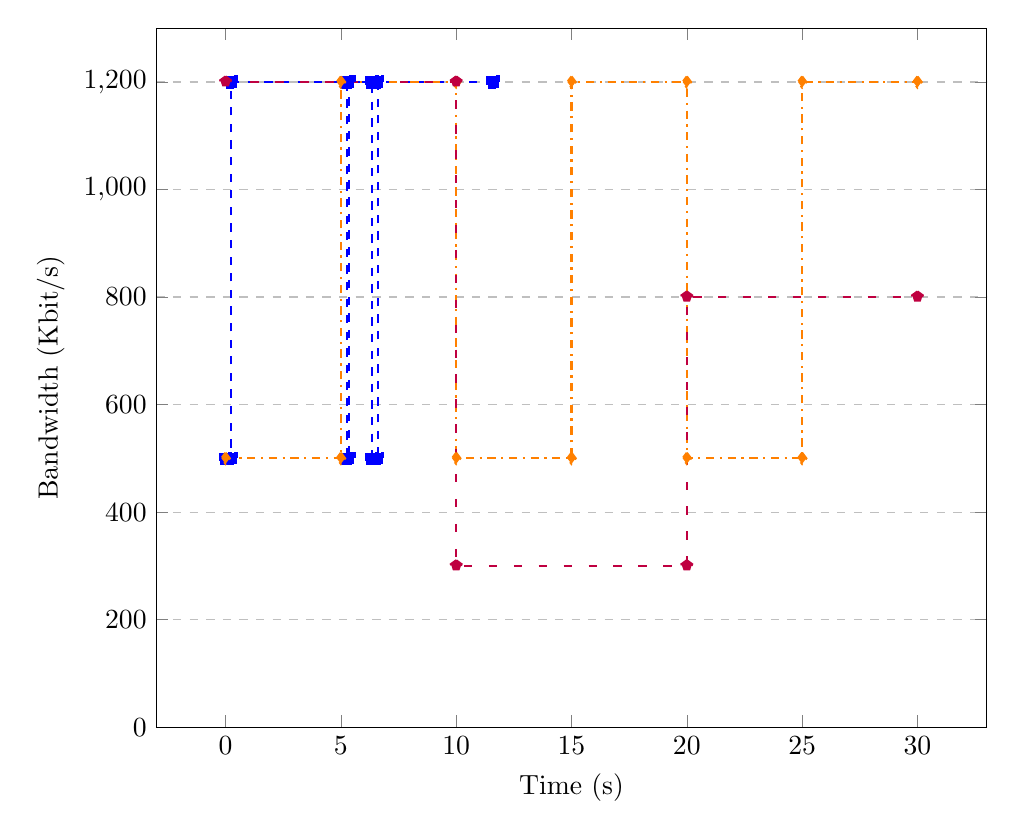
\begin{tikzpicture}
    \begin{axis}[
        width=\textwidth,
        xlabel={Time (s)},
        ylabel={Bandwidth (Kbit/s)},
        ymin=0, ymax=1300, ytick distance=200,
        ymajorgrids=true,
        grid style=dashed,
    ]

% FAST_JITTERS
\addplot[blue, const plot, thick, dashed, mark=square*] coordinates {
    (0,500) (0.25,500) (0.25,1200) (5.25,1200) (5.25,500) (5.35,500)
    (5.35,1200) (6.35,1200) (6.35,500) (6.6,500) (6.6,1200) (11.6,1200)
};

% SLOW_JITTERS
\addplot[orange, const plot, thick, dashdotted, mark=diamond*] coordinates {
    (0,500) (5,500) (5,1200) (10,1200) (10,500) (15,500) (15,1200) (20,1200)
    (20,500) (25,500) (25,1200) (30,1200)
};

% SPIKE
\addplot[purple, const plot, thick, loosely dashed, mark=pentagon*] coordinates {
    (0,1200) (10,1200) (10,300) (20,300) (20,800) (30,800)
};
        
\end{axis}
\end{tikzpicture}
\caption{Jitter profiles}
\label{fig:bandwidth_profiles:jitters}
\end{subfigure}
\end{figure}